\documentclass{standalone}
\usepackage[centertags]{amsmath}
\usepackage{latexsym}
\usepackage{amsfonts}
\usepackage{amssymb}
\usepackage{amsthm}
\usepackage{newlfont}
\usepackage{enumerate}
\usepackage{makeidx}
\usepackage{tikz}
\usepackage{nicematrix}

\usetikzlibrary{matrix,fit,positioning,arrows.meta}

\begin{document}
    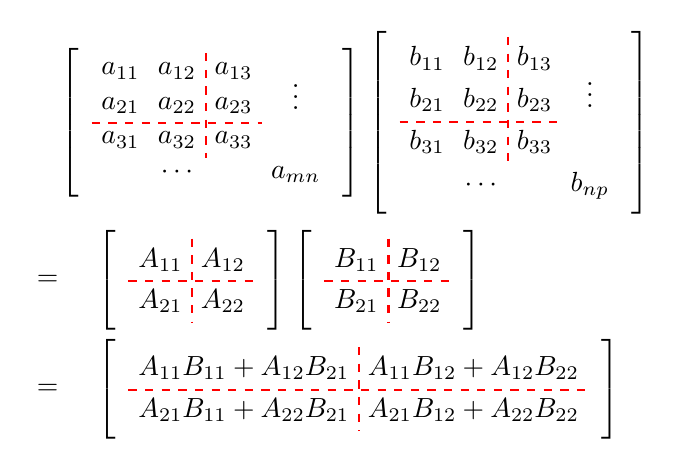
\begin{tikzpicture}
   \matrix (A) [matrix of math nodes,left delimiter=\lbrack,right delimiter=\rbrack]
{
a_{11} & a_{12} & a_{13} & \ \\
a_{21} & a_{22} & a_{23}  & \smash{\vdots} \\
a_{31} & a_{32} & a_{33} &  \\
& \cdots & \ & a_{mn} \\
};
   \matrix (B) [matrix of math nodes,left delimiter=\lbrack,right delimiter=\rbrack,xshift=-1em,right = of A]
{
b_{11} & b_{12} & b_{13} & \ \\
b_{21} & b_{22} & b_{23} & \smash{\vdots} \\
b_{31} & b_{32} & b_{33} & \\
& \cdots & \ & b_{np} \\
};
\node(eq1)[below= of A.south west,anchor=west,xshift=-2em]{=};
   \matrix (A2) [matrix of math nodes,left delimiter=\lbrack,right delimiter=\rbrack,xshift=-1em,right = of eq1]
{
A_{11} & A_{12}   \\
A_{21} & A_{22}   \\
};
   \matrix (B2) [matrix of math nodes,left delimiter=\lbrack,right delimiter=\rbrack,xshift=-1em,right = of A2]
{
B_{11} & B_{12}   \\
B_{21} & B_{22}   \\
};



\node(eq2)[below= of eq1.south]{=};
   \matrix (C) [matrix of math nodes,left delimiter=\lbrack,right delimiter=\rbrack,xshift=-1em,right = of eq2]
{
	A_{11}B_{11}+A_{12}B_{21} & A_{11}B_{12}+A_{12}B_{22}   \\
	    A_{21}B_{11}+A_{22}B_{21} & A_{21}B_{12}+A_{22}B_{22}   \\
};

\draw[thick,red,dashed] (A-1-2.north east) -- (A-3-2.south east); 
\draw[thick,red,dashed] (A-2-1.south west) -- (A-2-3.south east); 

\draw[thick,red,dashed] (B-1-2.north east) -- (B-3-2.south east); 
\draw[thick,red,dashed] (B-2-1.south west) -- (B-2-3.south east); 

\draw[thick,red,dashed] (A2-1-1.south west) -- (A2-1-2.south east); 
\draw[thick,red,dashed] (A2-1-1.north east) -- (A2-2-1.south east); 

\draw[thick,red,dashed] (B2-1-1.south west) -- (B2-1-2.south east); 
\draw[thick,red,dashed] (B2-1-1.north east) -- (B2-2-1.south east); 

\draw[thick,red,dashed] (C-1-1.south west) -- (C-1-2.south east); 
\draw[thick,red,dashed] (C-1-1.north east) -- (C-2-1.south east); 
    \end{tikzpicture}
\end{document}
